\documentclass{standalone}
\standaloneconfig{border=2mm 2mm 2mm 2mm}

\usepackage{mathtools}
\usepackage{amsmath}
\usepackage{amssymb}
\usepackage{amsfonts}

\usepackage{tikz}
\usepackage{scalerel}
\usepackage{pict2e}
\usepackage{tkz-euclide}
\usepackage{booktabs}
\usetikzlibrary{calc}
\usetikzlibrary{patterns, arrows.meta}
\usetikzlibrary{shadows}
\usetikzlibrary{external}
\usetikzlibrary{angles, quotes}

\begin{document}
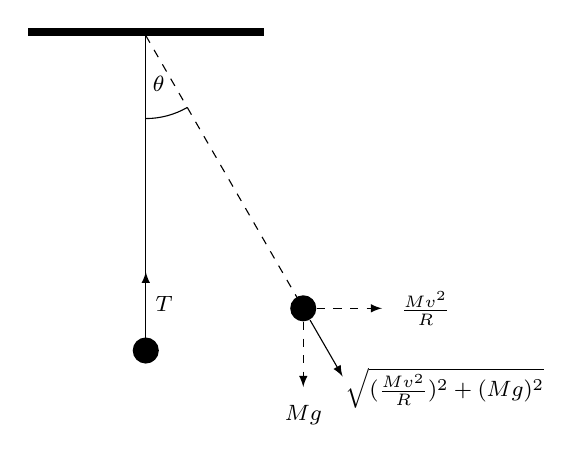
\begin{tikzpicture}[font=\footnotesize]

    \coordinate (a) at (0, 0);
    \coordinate (b) at (-60:2);
    \coordinate (c) at (-90:4);

    \fill (-1.5,0) rectangle(1.5,0.1);

    \draw (0,0) -- (-90:4) node[fill,circle](M){};

    \draw[dashed] (0,0) -- (-60:4) node[fill,circle](m){};

%    \draw[dashed] (0,0) -- (-60:2);

    \draw pic["$\theta$", draw, angle radius=30] {angle=c--a--b};

    \draw[dashed, -latex] (m) -- node[below=15pt]{$Mg$}++(0,-1) ;

    \draw [-latex] (M) -- node[right]{$T$}(-90:3);

    \draw[dashed, -latex] (m) -- node[right=15pt]{$\frac{Mv^2}{R}$}++(1,0);

    \draw[-latex] (m) -- node[below right = 5pt]{$\sqrt{(\frac{Mv^2}{R})^2 + (Mg)^2}$}++(-60:1);

%    \draw[-latex] (M) -- node[below right = 5pt]{$\frac{Mv^2}{R}\cos{\theta} + Mg\sin{\theta}$}++(-30:1);

\end{tikzpicture}
\end{document}